\documentclass{phyasgn}
\phyasgn{
  stuname = 姚昊廷,           % 设置学生姓名
  stunum = 22322091,      % 设置学号
  setasgnnum = 2,           % 设置课程次数
  classname = 电磁学,     % 设置课程名称
}

\usepackage{listings}
\usepackage{tikz}
\usepackage{amssymb}
\usepackage{t-angles}
\usepackage{amssymb}
\usepackage{tikz} 
\usetikzlibrary{quotes,angles}
\usetikzlibrary{calc}
\usetikzlibrary{decorations.pathreplacing}
\lstset{numbers=left,basicstyle=\ttfamily,columns=flexible}
\makeatletter
\newcommand{\rmnum}[1]{\romannumeral #1}
\newcommand{\Rmnum}[1]{\expandafter\@slowromancap\romannumeral #1@}
\makeatother


\begin{document}
{\zihao{5}\heiti\color{red} 1-9}
\begin{sol}
(1)
$$\mathrm{F}=\mathrm{F}_1+\mathrm{F}_2$$
$\mathrm{F}_1,\mathrm{F}_2$方向相反故
$$F=F_1-F_2$$
因为$l \ll r$,故$F_1-F_2=\frac{2Qql}{4\pi \varepsilon_0r^3}=\frac{2Qp}{4\pi \varepsilon_0r^3}$
因为$L_1=L_2=0$,故$L=0$
故$$\mathbf{F}=\frac{Q}{2\pi \varepsilon_0r^3}\mathbf{p}$$
$$\mathbf{L}=0$$
\par
(2)$$F_y=F_{1y}+F_{2y}=\frac{Qql}{4\pi \varepsilon_0r^3},F_x=F_{1x}-F_{2x}=0$$
$$\mathbf{F}=\frac{Q}{4\pi \varepsilon_0r^3}\mathbf{p}$$
$$L=F_{1x}\frac{l}{2}+F_{2x}\frac{l}{2}=\frac{Qp}{4\pi\varepsilon_0r^2}$$
故$$
\mathbf{L}=\frac{Q\mathbf{p}\times \mathbf{r}}{4\pi\varepsilon_0r^3}
$$
\end{sol}\par

{\zihao{5}\heiti\color{red} 1-13}
\begin{sol}
$$\begin{aligned}
    \phi&=\iint\limits_{x^2+y^2+z^2=a^2}\mathbf{E}\cdot\mathbf{n}\mathrm{d}S\\
    &=\iint\limits_{x^2+y^2\leq a^2}E\cos\theta\frac{\mathrm{d}x\mathrm{d}y}{\cos\theta}\\
    &=\iint\limits_{x^2+y^2\leq a^2}E\mathrm{d}x\mathrm{d}y\\
    &=E\pi a^2
\end{aligned}$$
\end{sol}\par

{\zihao{5}\heiti\color{red} 1-14}
\begin{sol}
取半径为$R$的球面,由于电荷分布是球对称的,故电场强度只有径向分量。
该闭合球面所包围的净电荷量为
$$\begin{aligned}
    q&=\int_{0}^{R}-\frac{e}{\pi a_B^3}\mathrm{e}^{-2r/a_B}4\pi r^2\mathrm{d}r+e\\
    &=\frac{e\mathrm{e}^{\frac{2R}{a_B}}(a_B^2+2a_B+2R^2)}{a_B^2}
\end{aligned}$$
由高斯定理
$$\begin{aligned}
    4\pi R^2E&=\frac{q}{\varepsilon_0}\\
    E&=\frac{e\mathrm{e}^{\frac{2R}{a_B}}(a_B^2+2a_B+2R^2)}{4\pi\varepsilon_0a_B^2R^2}
\end{aligned}$$
方向为由原子中心指向外面
\end{sol}\par

{\zihao{5}\heiti\color{red} 1-15}
\begin{sol}
(1)
取底面为面元$\mathrm{d}S$的闭合柱面,则该曲面电通量为
$$\phi=(E_1-E_2)\mathrm{d}S$$
由高斯定理
$$\phi=\frac{q}{\varepsilon_0}=\frac{\rho \mathrm{d}S h}{\varepsilon_0}$$
则$$\rho=\frac{(E_1-E_2)\varepsilon_0}{h}=4.43\times 10^{-13}C/m^3$$
(2)$$\begin{aligned}
    \frac{4\pi R^2\sigma}{\varepsilon_0}&=-4\pi R^2E_1\\
    \sigma&=-\varepsilon_0E_1=-8.85\times 10^{-10}C/m^2
\end{aligned}$$
\end{sol}\par

{\zihao{5}\heiti\color{red} 1-12}
\begin{sol}
    设两条直线如图放置,取两线中点为坐标原点
    \begin{figure}[htbp]
        \begin{tikzpicture}
            \draw (0,0) --(0,5) node[above] {+};
            \draw (2,0) --(2,5) node[above] {-};
            \draw[->] (-3,2.5) --(5,2.5) node[right] {$x$};
            \filldraw (1,2.5) circle (.1) node[below] {$O$};
        \end{tikzpicture}
    \end{figure}
    
(1)设$\hat{x}$为沿$x$轴正方向的单位矢量由场强叠加原理知当$x<-\frac{a}{2}$时场强为
$$
\mathbf{E}=\frac{\eta_e}{2\pi\varepsilon_0(-\frac{a}{2}-x)}(-\hat{x})+\frac{\eta_e}{2\pi\varepsilon_0(\frac{a}{2}-x)}\hat{x}=\frac{-a\eta_e}{2\pi\varepsilon_0(x^2-\frac{a^2}{4})}\hat{x}
$$
当$-\frac{a}{2}<x<\frac{a}{2}$时场强为
$$
\mathbf{E}=\frac{\eta_e}{2\pi\varepsilon_0(x+\frac{a}{2})}\hat{x}+\frac{\eta_e}{2\pi\varepsilon_0(\frac{a}{2}-x)}\hat{x}=\frac{-a\eta_e}{2\pi\varepsilon_0(x^2-\frac{a^2}{4})}\hat{x}
$$
当$\frac{a}{2}<x$时场强为
$$
\mathbf{E}=\frac{\eta_e}{2\pi\varepsilon_0(x+\frac{a}{2})}\hat{x}+\frac{\eta_e}{2\pi\varepsilon_0(x-\frac{a}{2})}(-\hat{x})=\frac{-a\eta_e}{2\pi\varepsilon_0(x^2-\frac{a^2}{4})}\hat{x}
$$
综上$$
\mathbf{E}=\frac{\eta_e}{2\pi\varepsilon_0(x+\frac{a}{2})}\hat{x}+\frac{\eta_e}{2\pi\varepsilon_0(x-\frac{a}{2})}(-\hat{x})=\frac{-a\eta_e}{2\pi\varepsilon_0(x^2-\frac{a^2}{4})}\hat{x}
$$
\par
(2)$$
F=\eta_e\cdot\frac{\eta_e}{2\pi\varepsilon_0a}=\frac{\eta_e^2}{2\pi\varepsilon_0a}
$$
\end{sol}\par

{\zihao{5}\heiti\color{red} 1-16}
\begin{sol}
    由对称性知,场强方向定垂直于轴线,取以轴线为中心线半径为$r$长为$l$的圆柱形高斯面可得
    $$
        2\pi rlE=\frac{q}{\varepsilon_0}
    $$
    又$r<R$时$q=0$,故$E=0$。$r>R$时$q=l\lambda$故$E=\frac{\lambda}{2\pi\varepsilon_0r}$。\\
    当$r=R$时高斯定律不适用,可将圆筒沿轴线方向分为无数带电直线
    \begin{figure}[htbp]
        \begin{tikzpicture}
            \coordinate (o) at (5,5);
            \coordinate (a) at (0.175,6.311);
            \coordinate (b) at (0.6695,7.499);
            \coordinate (p) at (5,0);
            \coordinate (c) at (5,10);
            \draw (o) circle (5);
            \draw (p) --(c);
            \draw (p) --(a);
            \draw (b) --(p) node[below] {$P$};
            \draw[loosely dashed] (o) --(a) ;
            \draw[loosely dashed] (o) --(b);
            
            \pic["$2\mathrm{d}\theta$", draw=green!40, <->, angle eccentricity=0.6, angle radius=1.5cm]
            {angle=b--o--a};
            \pic["$\mathrm{d}\theta$", draw=green!40, <->, angle eccentricity=0.6, angle radius=1.5cm]
            {angle=b--p--a};
            \pic["$\theta$", draw=green!40, <->, angle eccentricity=0.6, angle radius=3cm]
            {angle=c--p--a};
        \end{tikzpicture}
    \end{figure}\\
    每一带电直线的电荷线密度为$\lambda_0=\frac{2\mathrm{d}\theta}{2\pi}\lambda$,于是在$P$点产生的场强就为
    $$
        \mathrm{d}E=\frac{\lambda_0}{2\pi\varepsilon_0r}
    $$
    又因为$r=2R\cos\theta$
    故$$
    \mathrm{d}E=\frac{\lambda\mathrm{d}\theta}{4\pi^2\varepsilon_0R\cos\theta}
    $$
    其径向分量为$\mathrm{d}E\cos\theta=\frac{\lambda\mathrm{d}\theta}{4\pi^2\varepsilon_0R}$
    故$$
        E=2\int_0^{\frac{\pi}{2}}\frac{\lambda\mathrm{d}\theta}{4\pi^2\varepsilon_0R}=\frac{\lambda}{4\pi\varepsilon_0R}
    $$
    故$$
    E=\left\{\begin{matrix}
        0&(r<R) \\
        \frac{\lambda}{4\pi\varepsilon_0R} &(r=R) \\
        \frac{\lambda}{2\pi\varepsilon_0r}&(r>R)
      \end{matrix}\right.
    $$
    $E-r$图为\\
    \begin{figure}[htbp]
        \begin{tikzpicture}
            \draw[->] (0,0) --(6,0) node[right] {$r$};
    \draw[->] (0,0) --(0,3) node[above] {$E$};
    \draw[loosely dashed] (0.5,3) --(0.5,0) node[below] {$R$};
    \draw[loosely dashed] (0.5,2) --(0,2) node[left] {$\frac{\lambda}{2\pi\varepsilon_0R}$};
    \draw (0.5,2) circle (.1);
    \filldraw (0.5,1) circle (.1);
    \draw[loosely dashed] (0.5,1) --(0,1) node[left] {$\frac{\lambda}{4\pi\varepsilon_0R}$};
    \draw[domain =0.5:5] plot (\x ,{1/\x}) ;
        \end{tikzpicture}
    \end{figure}
\end{sol}\par

{\zihao{5}\heiti\color{red} 1-19}
\begin{sol}
    不妨设三个平面如图分布将空间分为\Rmnum{1},\Rmnum{2},\Rmnum{3},\Rmnum{4}四部分。且令$\sigma_e>0$\newpage
    \begin{figure}[htbp]
        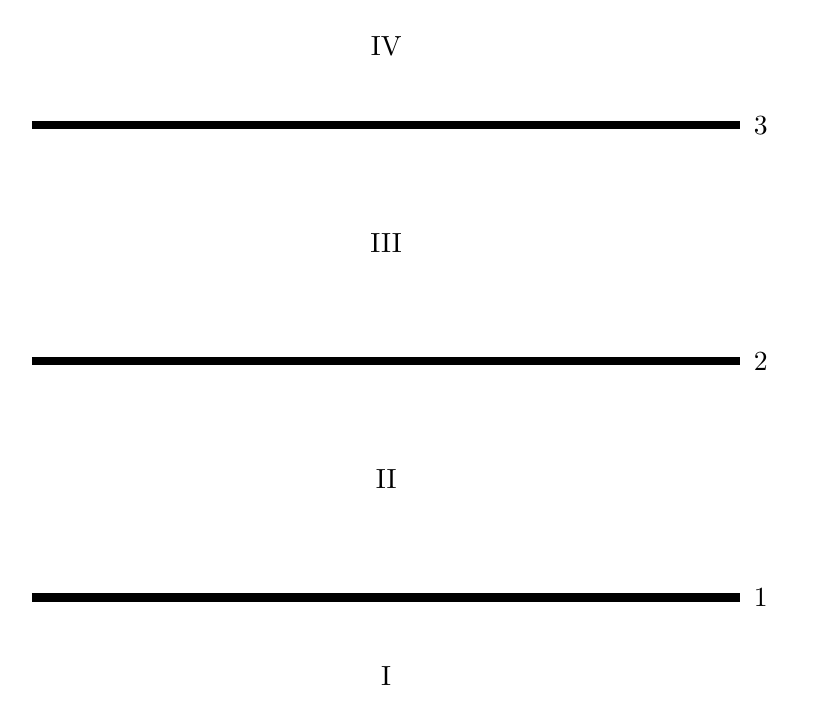
\begin{tikzpicture}
            \node at(4.5,2) {\Rmnum{1}};
            \draw [line width =3pt] (0,3)--(9,3) node[right] {1};
            
            \node at(4.5,4.5) {\Rmnum{2}};
            \draw [line width =3pt] (0,6)--(9,6) node[right] {2};
            
            \node at(4.5,7.5) {\Rmnum{3}};
            \draw [line width =3pt] (0,9)--(9,9) node[right] {3};
            
            \node at(4.5,10) {\Rmnum{4}};
        \end{tikzpicture}
    \end{figure}\par
    
由场强叠加原理知\\
(1)$E_{\rmnum{1}}=\frac{3\sigma_e}{2\varepsilon_0},E_{\rmnum{2}}=\frac{\sigma_e}{2\varepsilon_0},E_{\rmnum{3}}=\frac{\sigma_e}{2\varepsilon_0},E_{\rmnum{4}}=\frac{3\sigma_e}{2\varepsilon_0}$\\
方向分别为下下上上\\
(2)$E_{\rmnum{1}}=\frac{\sigma_e}{2\varepsilon_0},E_{\rmnum{2}}=\frac{\sigma_e}{2\varepsilon_0},E_{\rmnum{3}}=\frac{\sigma_e}{2\varepsilon_0},E_{\rmnum{4}}=\frac{\sigma_e}{2\varepsilon_0}$\\
方向分别为下上下上\\
(3)$E_{\rmnum{1}}=\frac{\sigma_e}{2\varepsilon_0},E_{\rmnum{2}}=\frac{\sigma_e}{2\varepsilon_0},E_{\rmnum{3}}=\frac{\sigma_e}{2\varepsilon_0},E_{\rmnum{4}}=\frac{\sigma_e}{2\varepsilon_0}$\\
方向分别为上下上下\\
(4)$E_{\rmnum{1}}=\frac{\sigma_e}{2\varepsilon_0},E_{\rmnum{2}}=\frac{3\sigma_e}{2\varepsilon_0},E_{\rmnum{3}}=\frac{\sigma_e}{2\varepsilon_0},E_{\rmnum{4}}=\frac{3\sigma_e}{2\varepsilon_0}$\\
方向分别为上上上下\\
\end{sol}\par

\end{document}